\chapter{Zusammenspiel mit anderen Anwendungen und Programmen}
\label{ch:exportImport}
\label{sec:EExpo}

\section{Literaturlisten exportieren}
\label{sec:llExportieren}
PUMA ermöglicht einen Export\index{Export} von Publikationslisten aus PUMA in andere Programme.
Der Export erfolgt in zwei Schritten. Es wird zuerst ein Literaturverzeichnis in Puma zusammengestellt und exportiert, bevor es dann in ein anderes Programm importiert wird.
Um ein Literaturverzeichnis zusammenzustellen, müssen im ersten Schritt die Publikationen, die exportiert werden sollen, in die Ablage kopiert werden (vgl. \autoref{sec:ablage}).
		
\begin{figure}[h!]
 \centering
 \fbox{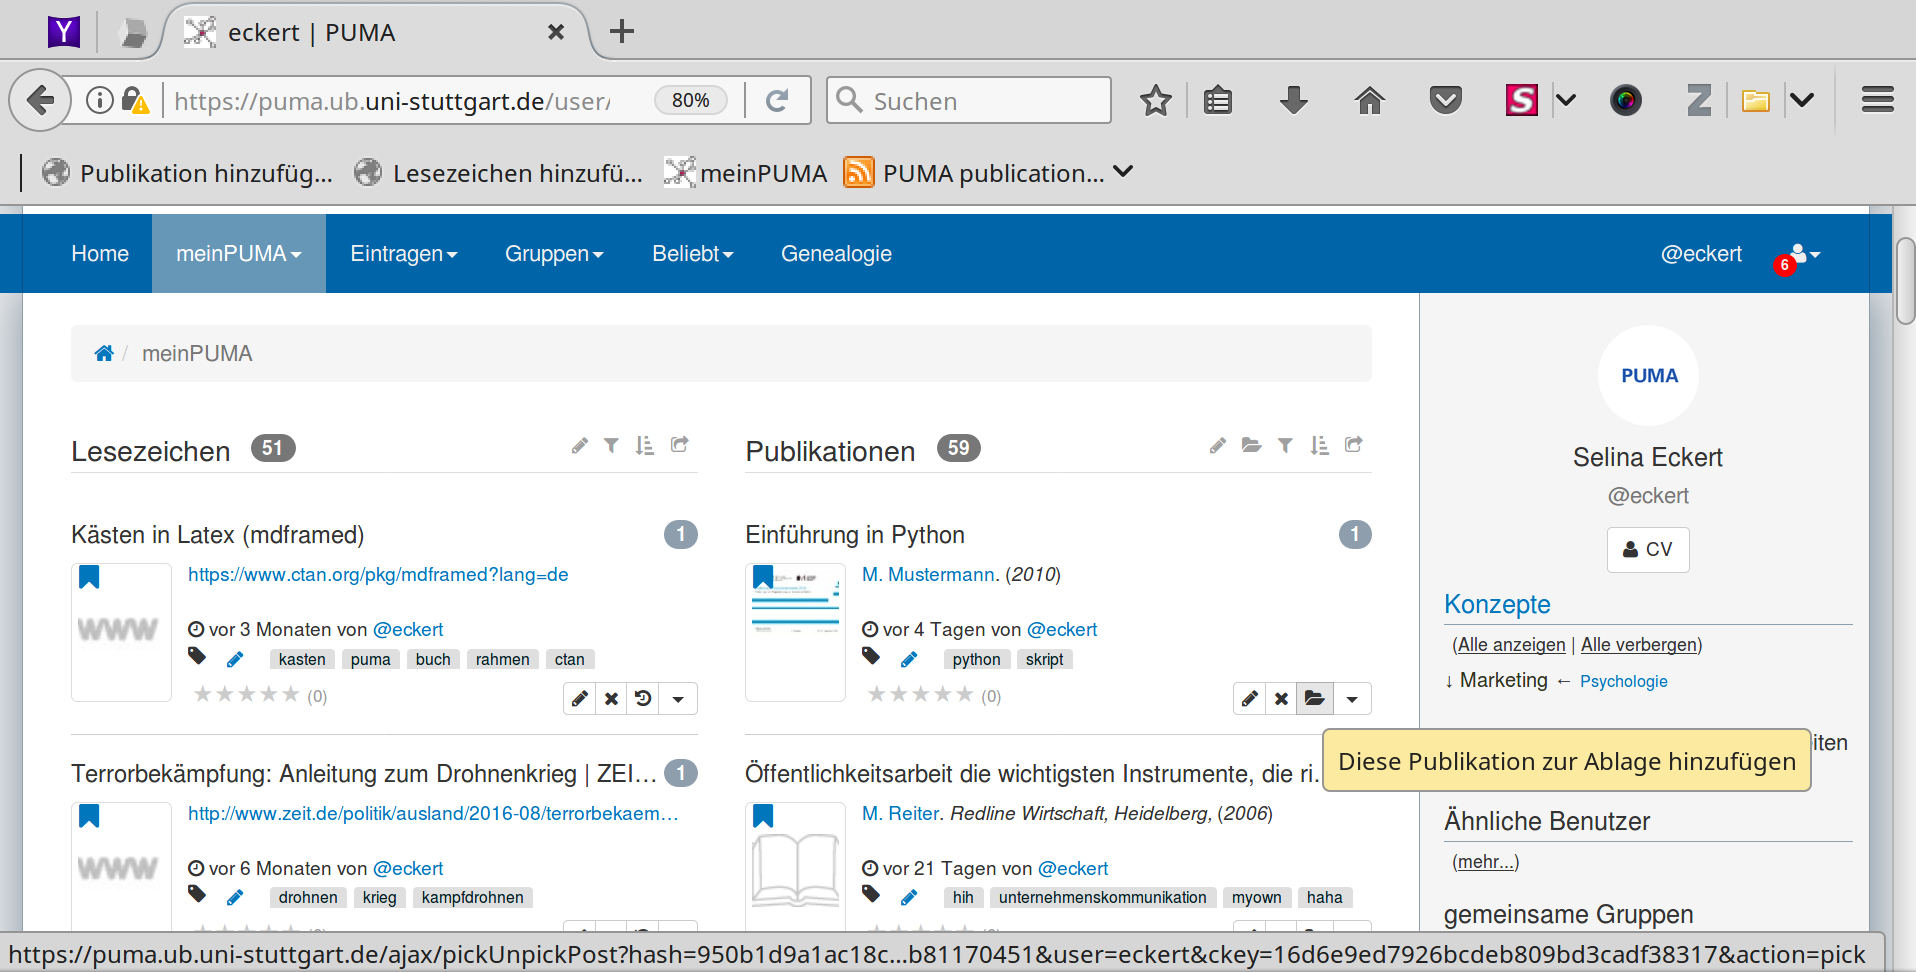
\includegraphics[width=10cm]{Bilder/Kapitel7/Zur_Ablage_hinzufuegen}}
 \caption{Zur Ablage hinzufügen}
 \label{fig:zurAblageHinzu}
\end{figure}

In der Ablage über das Exportzeichen oben rechts das Format, in dem das Literaturverzeichnis exportiert werden soll auswählen. Über \enquote{mehr...} stehen weitere Exportformaten zur Verfügung. Sollte das gewünschte Format nicht dabei sein, kann auch ein eigenes generiert werden (vgl. \todo{Verweis}).
\begin{figure}[h!]
 \centering
 \fbox{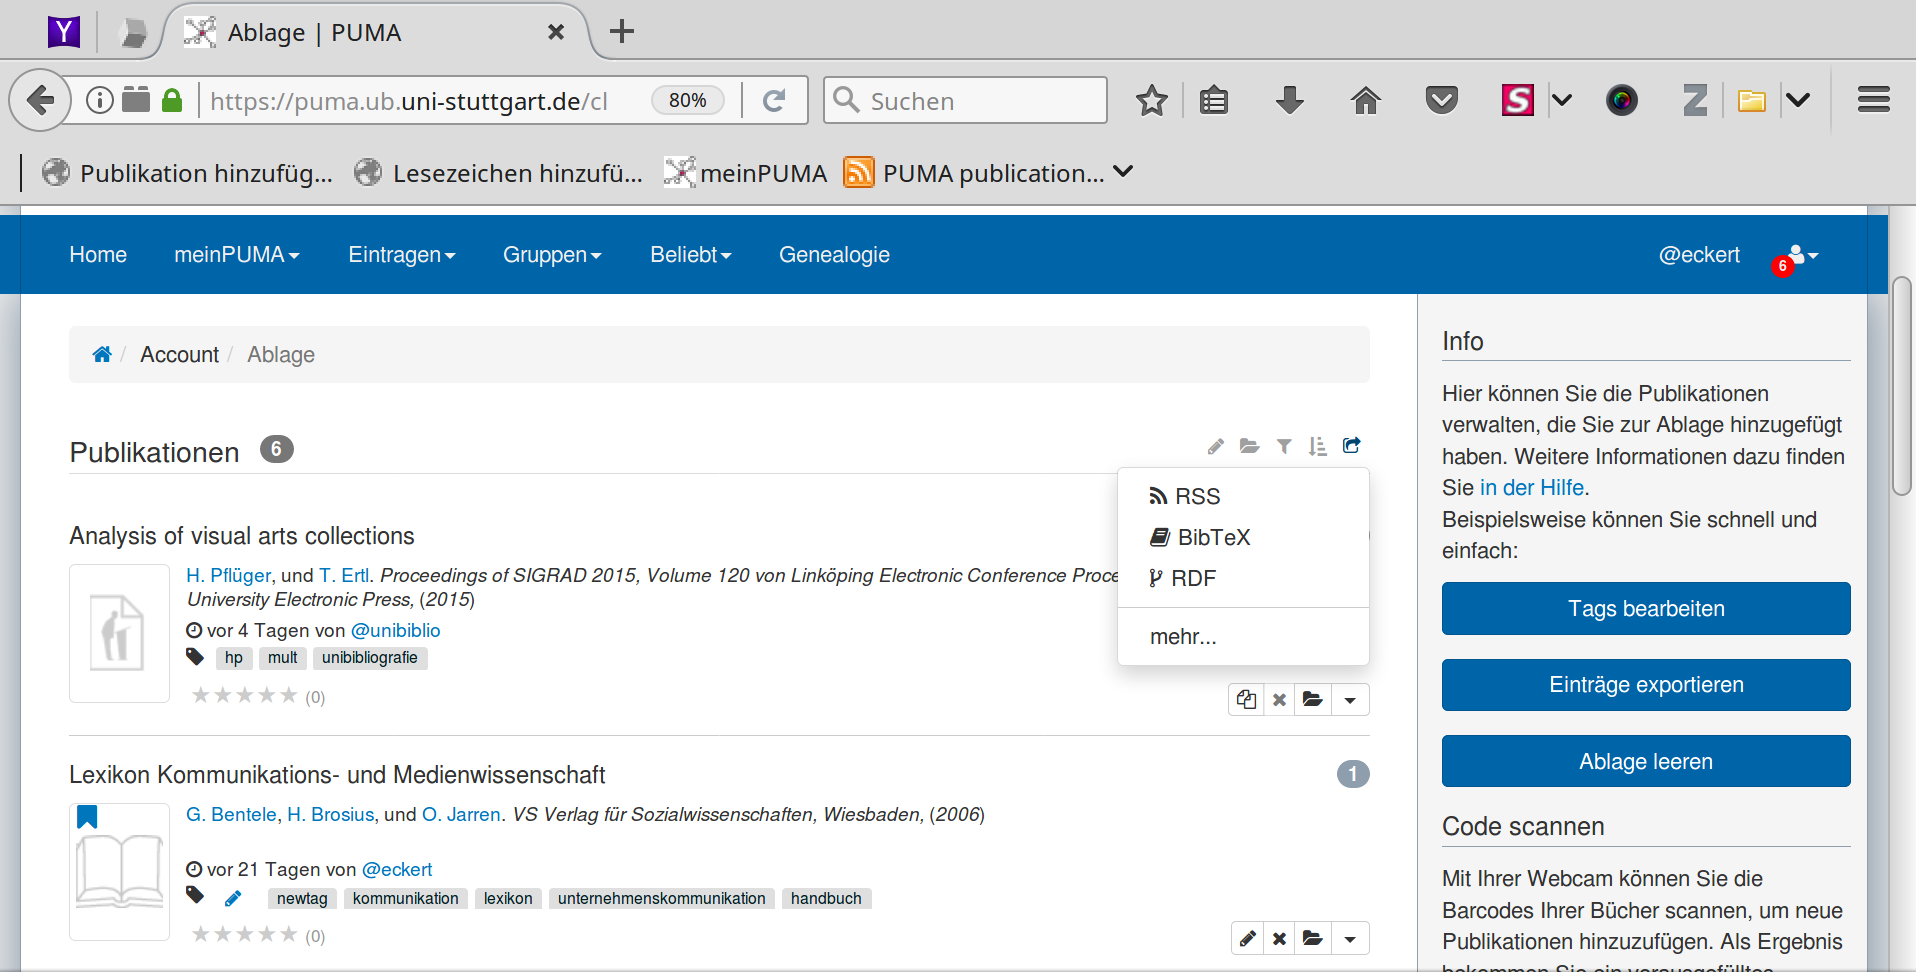
\includegraphics[width=11cm]{Bilder/Kapitel7/Exportformat_auswaehlen}}
 \caption{Das Exportformat auswählen}
 \label{fig:exportformatAuswaehlen}
\end{figure}


		
\begin{figure}[h!]
 \centering
 \fbox{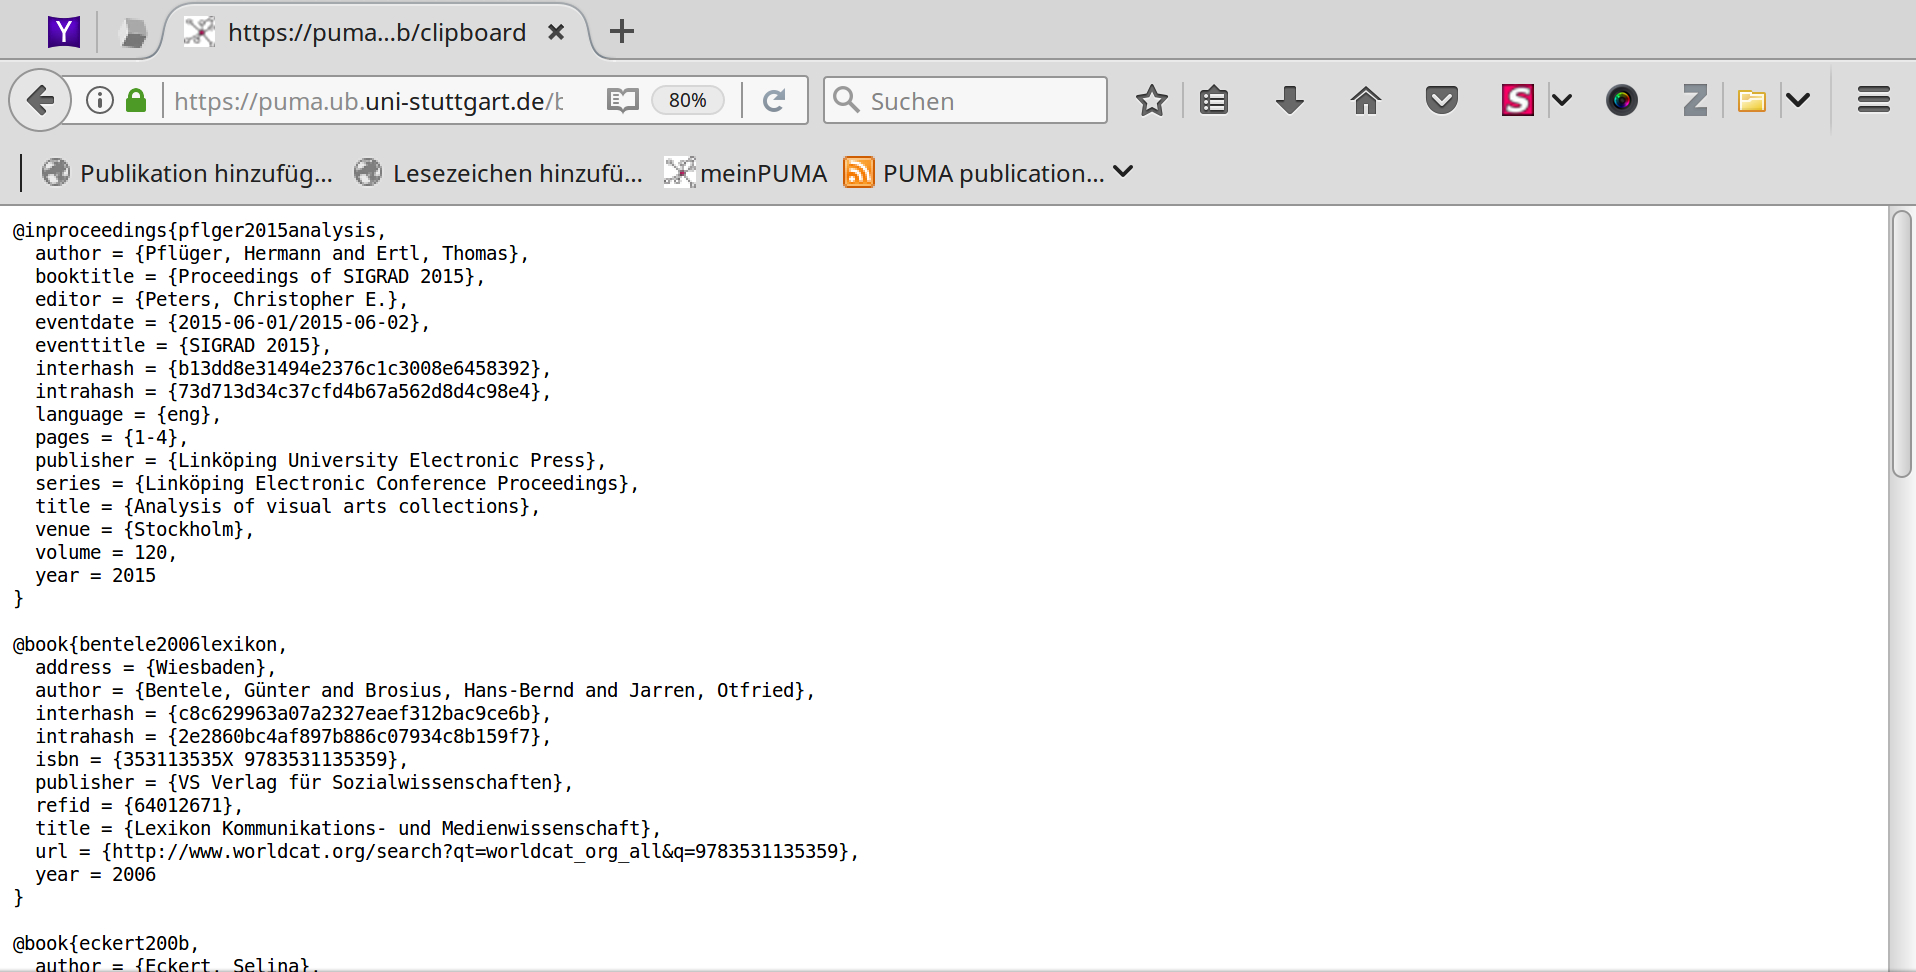
\includegraphics[width=11cm]{Bilder/Kapitel7/Das_Literaturverzeichnis}}
 \caption{Das Literaturverzeichnis}
 \label{fig:literaturverzeichnis}
\end{figure}


\subsection{Literaturverzeichnis exportieren - Programmspezifisch}
\label{subsec:lvExportProgramme}
\subsubsection*{Export nach Word\index{Export!Word}} \index{Word} \label{sss:exportWord}
In Microsoft Word kann die, im Format \enquote{MSOffice XML} \index{MSOffice XML} gespeicherte Datei verwendet werden, indem im Quellen-Manager (\enquote{Verweise}\enquote{Quellen verwalten}) die gespeicherte Datei ausgewählt wird \footcite{Genaue Anleitung im Blogbeitrag:https://blog.ub.uni-stuttgart.de/category/puma/}{}.\todo[inline]{mir geht die Beschreibung zu weit. Ich würde bei PUMA aufhören.}
%\begin{enumerate}
    %\item Klicken Sie in der Ablage auf das Exportzeichen.
    %\item Wählen Sie im Dropdown-Menü \enquote{mehr...} aus.
    %\item Es öffnet sich die Übersichtsseite der Exportformate. . Speichern Sie anschließend die Datei.
\begin{figure}[h!]
 \centering
 \fbox{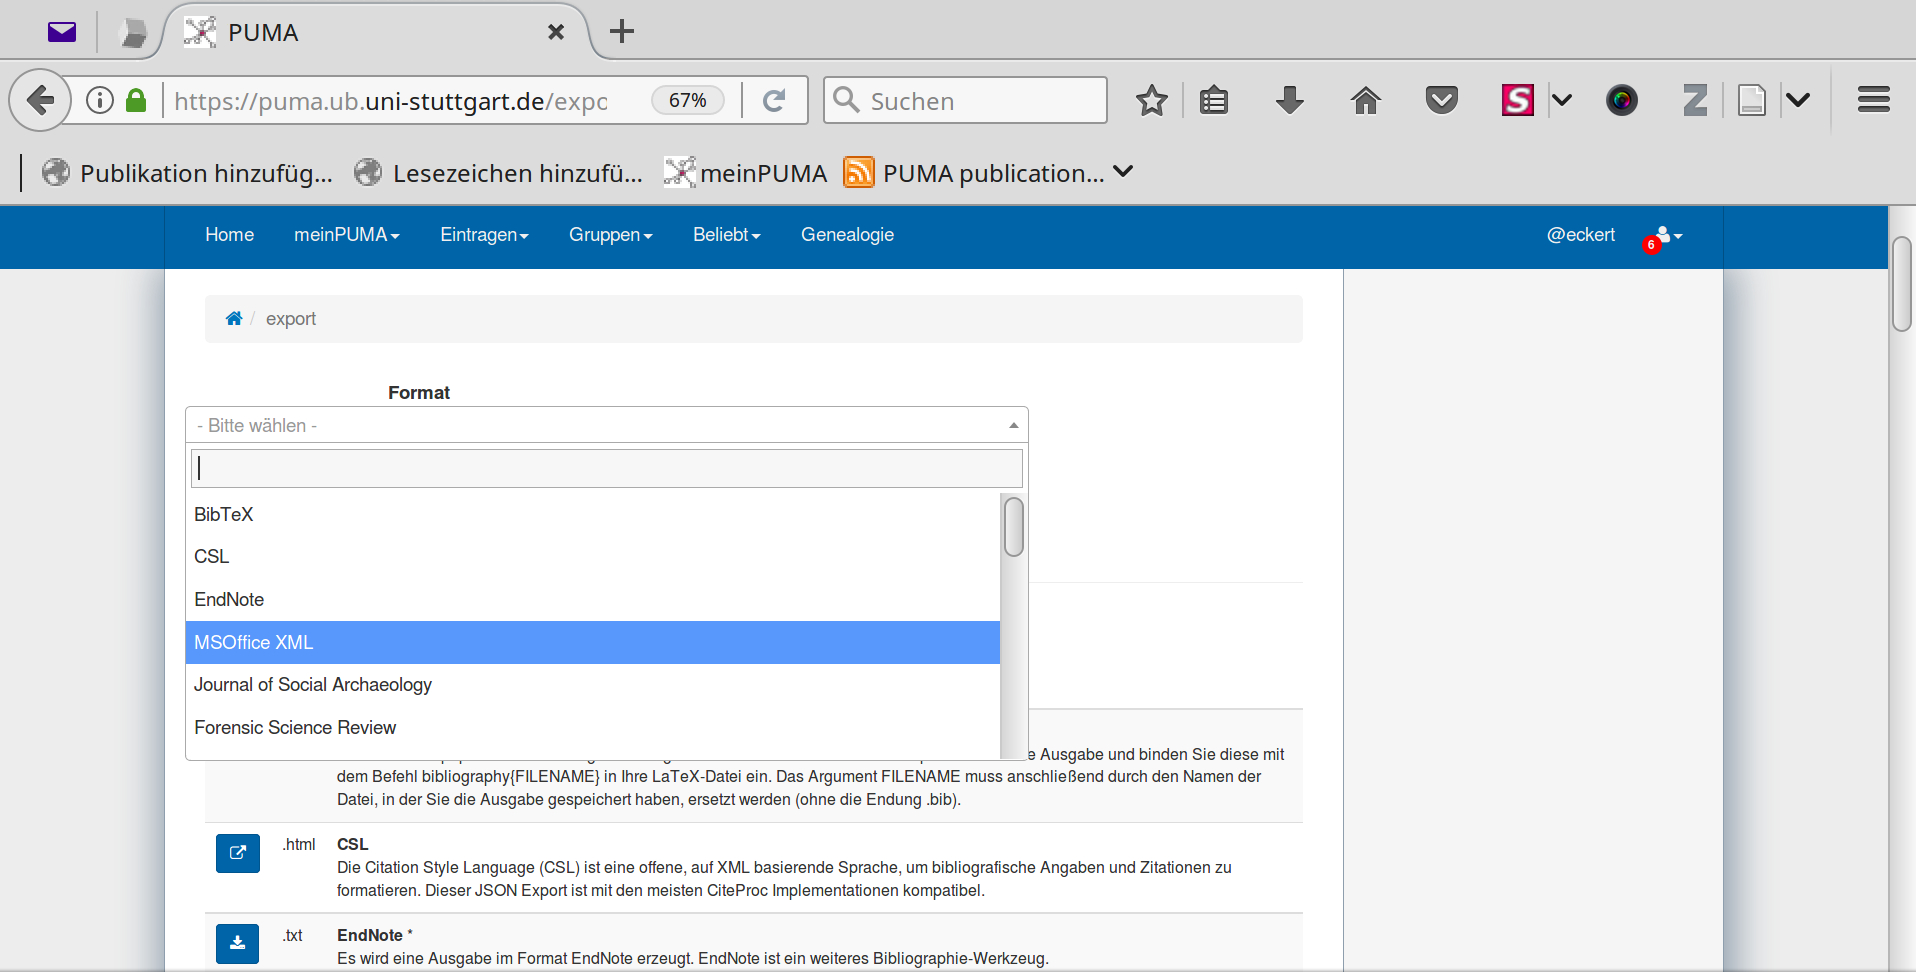
\includegraphics[width=11cm]{Bilder/Kapitel7/MSOffice_XML}}
 \caption{Das Exportformat MSOffice XML}
 \label{fig:exportformatMSOfficeXml}
\end{figure}

\begin{figure}[h!]
 \centering
 \fbox{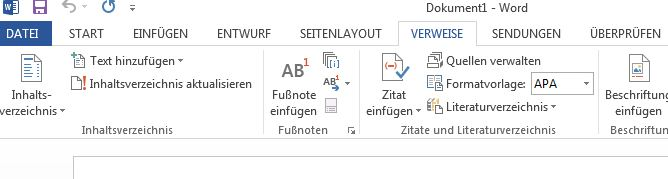
\includegraphics[width=11cm]{Bilder/Kapitel7/Word}}
 \caption{Reiter Verweise}
 \label{fig:reiterVerweise}
\end{figure}
\begin{figure}[h!]
 \centering
 \fbox{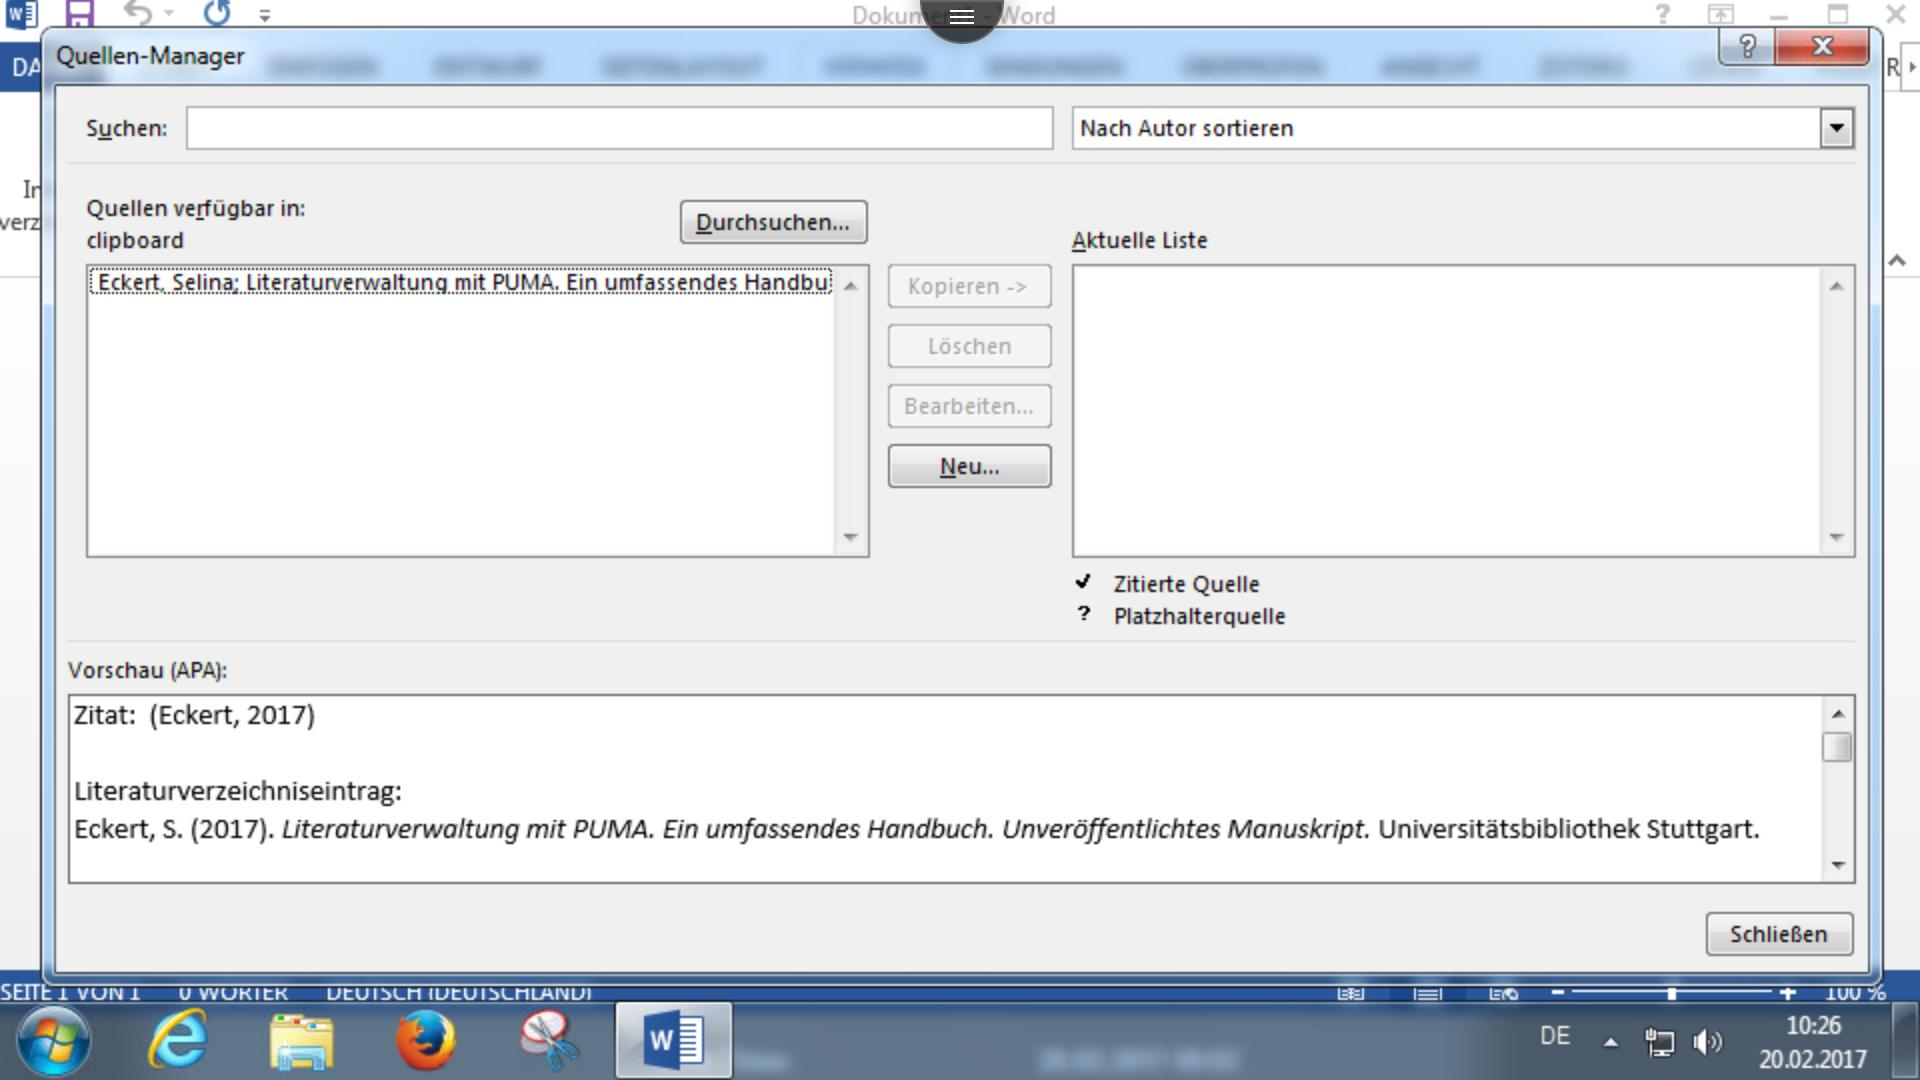
\includegraphics[width=11cm]{Bilder/Kapitel7/Quellen-Manager}}
 \caption{Quellen-Manager}
 \label{fig:quellenManager}
\end{figure} 

\subsubsection*{Export nach Citavi\index{Export!Citavi}}\label{sss:exportCitavi}
Für Citavi die Literaturliste in BibTeX exportieren und in die Zwischenablage kopieren. 
In Citavi in der Menüleiste oben links \enquote{Datei} auswählen und im Dropdown-Menü \enquote{Importieren} auswählen. 
Über \enquote{Aus einer Textdatei (Ris-, BibTex-formatiert o.ä.)} BibTeX als Format auswählen und anschließend über \enquote{Textdaten in der Zwischenablage verwenden} Datei hochladen. Die BibTeX-Keys über \enquote{Importierte BibTex Keys ersetzen} normalisieren und die \enquote{Titel übernehmen}.

\subsubsection*{Export nach Zotero\index{Export!Zotero}}\label{sss:exportZotero}
Auf der gewünschten PUMA-Seite, von der eine Publikation in die Zotero-Bibliothek übernommen werden soll, auf den schwarzen Pfeil neben dem Zotero\index{Zotero}-Symbol oben rechts bei Firefox.
Ein Dropdown-Menü öffnet sich. \enquote{In Zotero mit \enquote{unAPI} speichern} auswählen.
    
\begin{figure}[h!]
 \centering
 \fbox{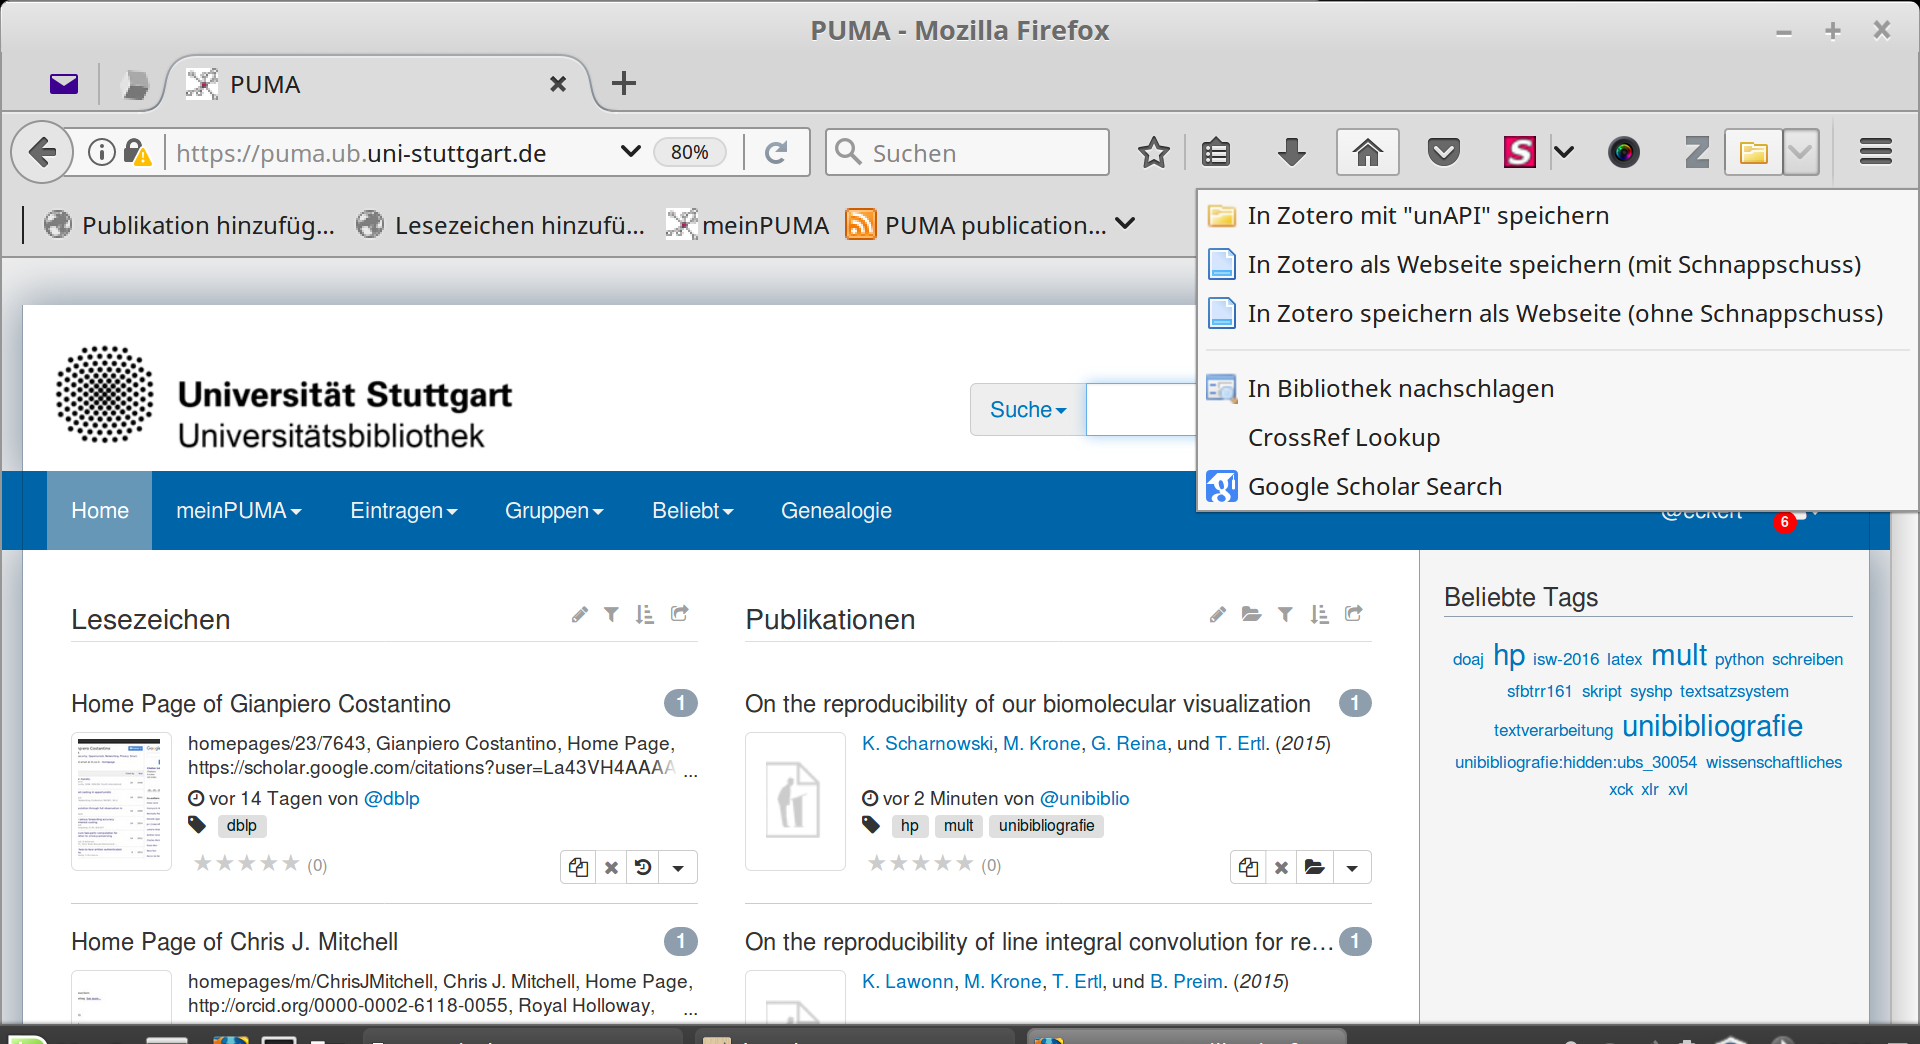
\includegraphics[width=10cm]{Bilder/Kapitel7/Zotero_Dropdown_Menue}}
 \caption{Dropdown-Menü}
 \label{fig:dropdownMenue}
\end{figure}

Es öffnet sich ein Popup-Fenster, in dem alle Publikationen der entsprechenden PUMA-Seite aufgelistet sind. Die Publikationen auswählen, die in die Zotero-Bibliothek übernommen werden sollen.
\begin{figure}[h!]
 \centering
 \fbox{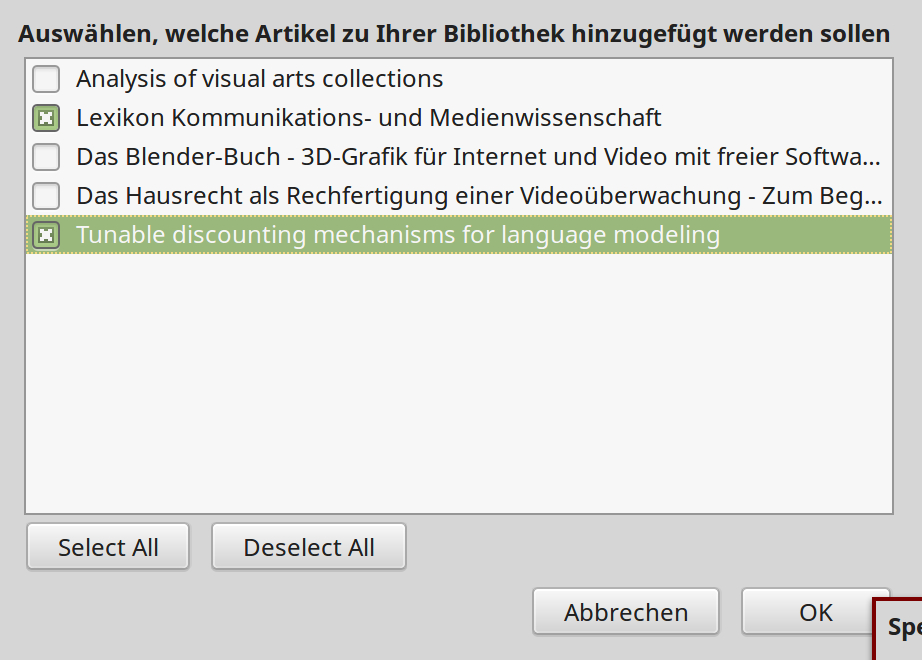
\includegraphics[width=10cm]{Bilder/Kapitel7/Zotero_Eintraege_auswaehlen}}
 \caption{Einträge auswählen}
 \label{fig:eintraegeAuswaehlen}
\end{figure}


\subsubsection*{Export nach JabRef\index{Export!JabRef}}\label{sss:exportJabref}
Für JabRef die Literaturliste in BibTeX exportieren und speichern. In JabRef dann die Datei über \enquote{Importieren in neue Datenbank} oder \enquote{Importieren in aktuelle Datenbank} importieren.

\section{Literaturlisten importieren}
\label{sec:llImportieren}
Das Importieren\index{Import} von Literaturlisten aus anderen Programmen in PUMA ist jederzeit möglich. Der Import erfolgt in zwei Schritten. Zuerst werden die gewünschten Publikationen aus dem Literaturverwaltungsprogramm exportiert, um dann anschließend in PUMA importiert zu werden. 
\subsection{BibTex-Export aus verwendeten Literaturverwaltungsprogrammen}
\label{subsec:bibtexExport}
\subsubsection*{Import aus Zotero\index{Import!Zotero}} \label{sss:importZotero}

Um den Import von Zotero\index{Zotero} zu PUMA zu ermöglichen, muss Zotero zunächst für PUMA konfiguriert werden:

Zotero öffnen und in den Einstellungen zu den Website-spezifischen Einstellungen einen neuen Eintrag hinzufügen. Dazu auf das \enquote{ '+'-Symbol}klicken und bei Domain/Pfad \textit{puma.ub.uni-stuttgart.de} eingeben und \textit{BibTeX\index{BibTex}} als Ausgabeformat auswählen.
\begin{figure}[h!]
 \centering
 \fbox{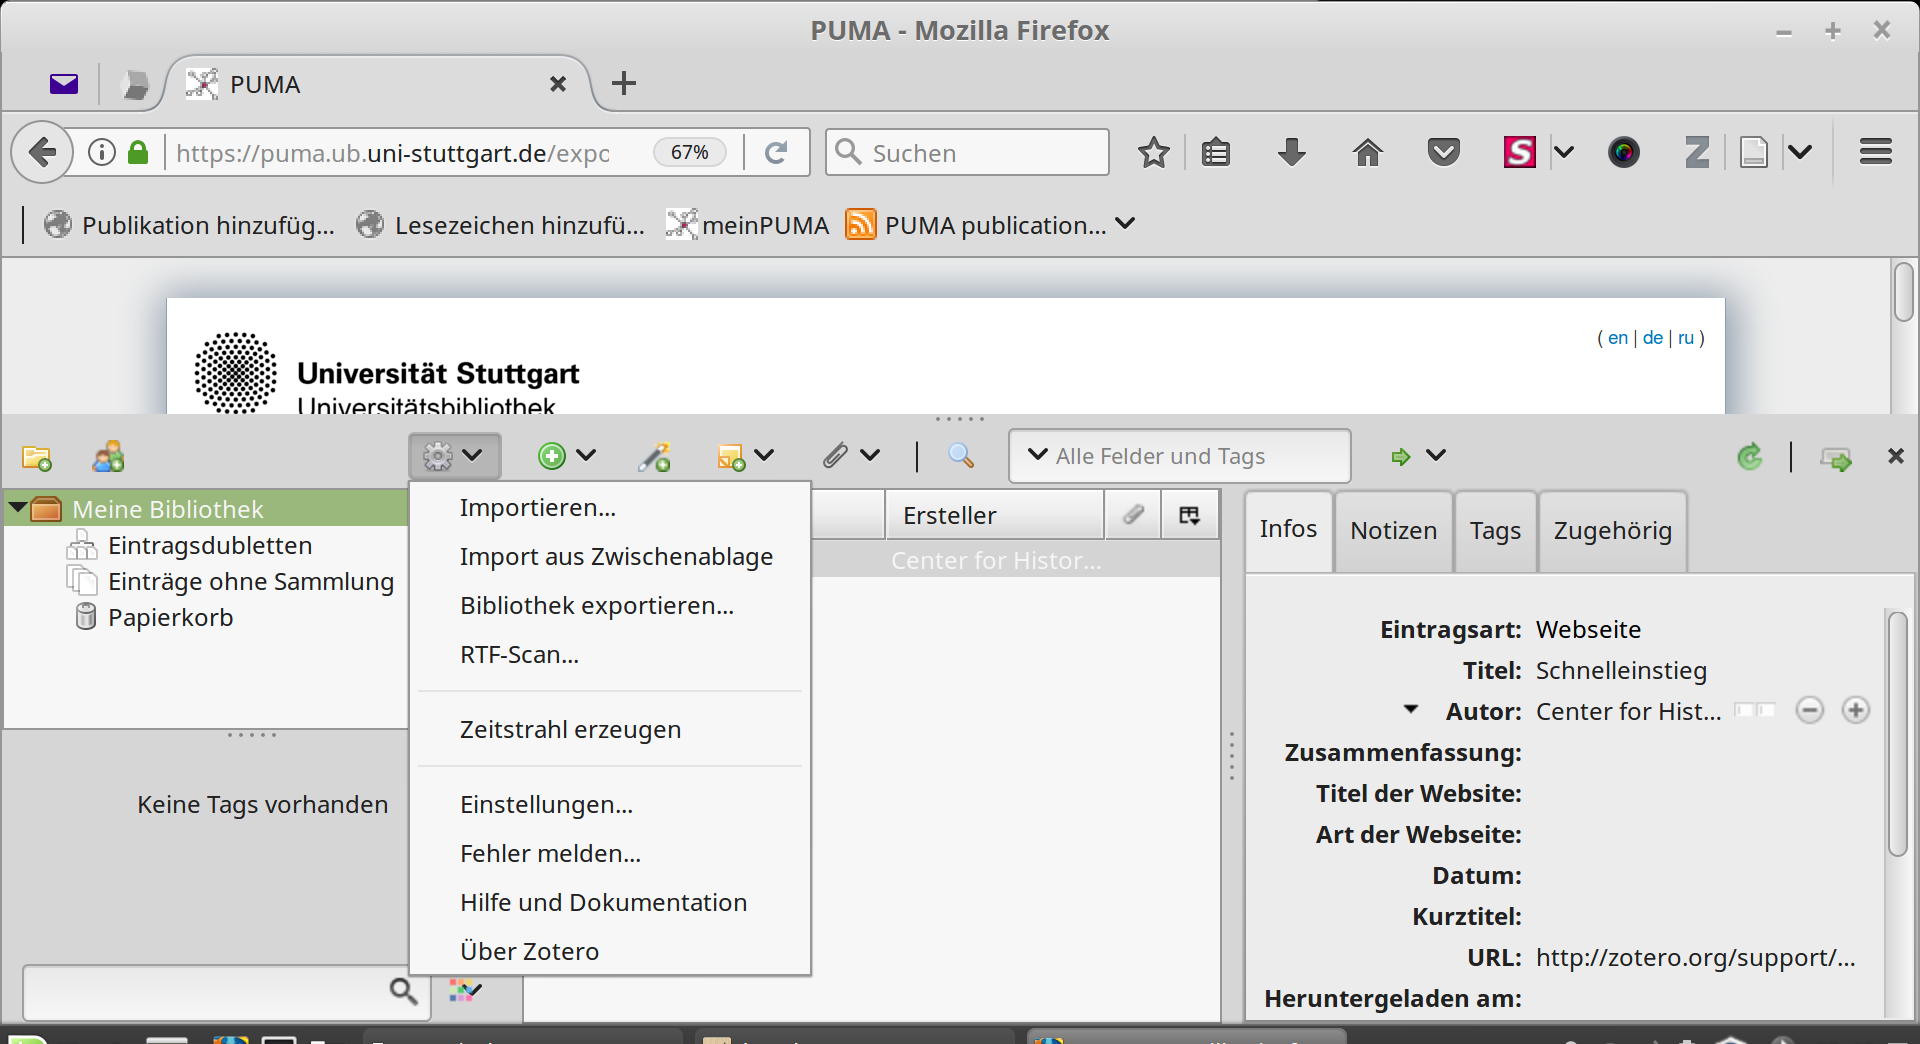
\includegraphics[width=9cm]{Bilder/Kapitel7/Zotero_Import}}
 \caption{Import aus Zotero}
 \label{fig:importZotero}
\end{figure}
Im Dropdown-Menü \enquote{Einstellungen} $/to$ \enquote{Export}auswählen.

\begin{figure}[h!]
 \centering
 \fbox{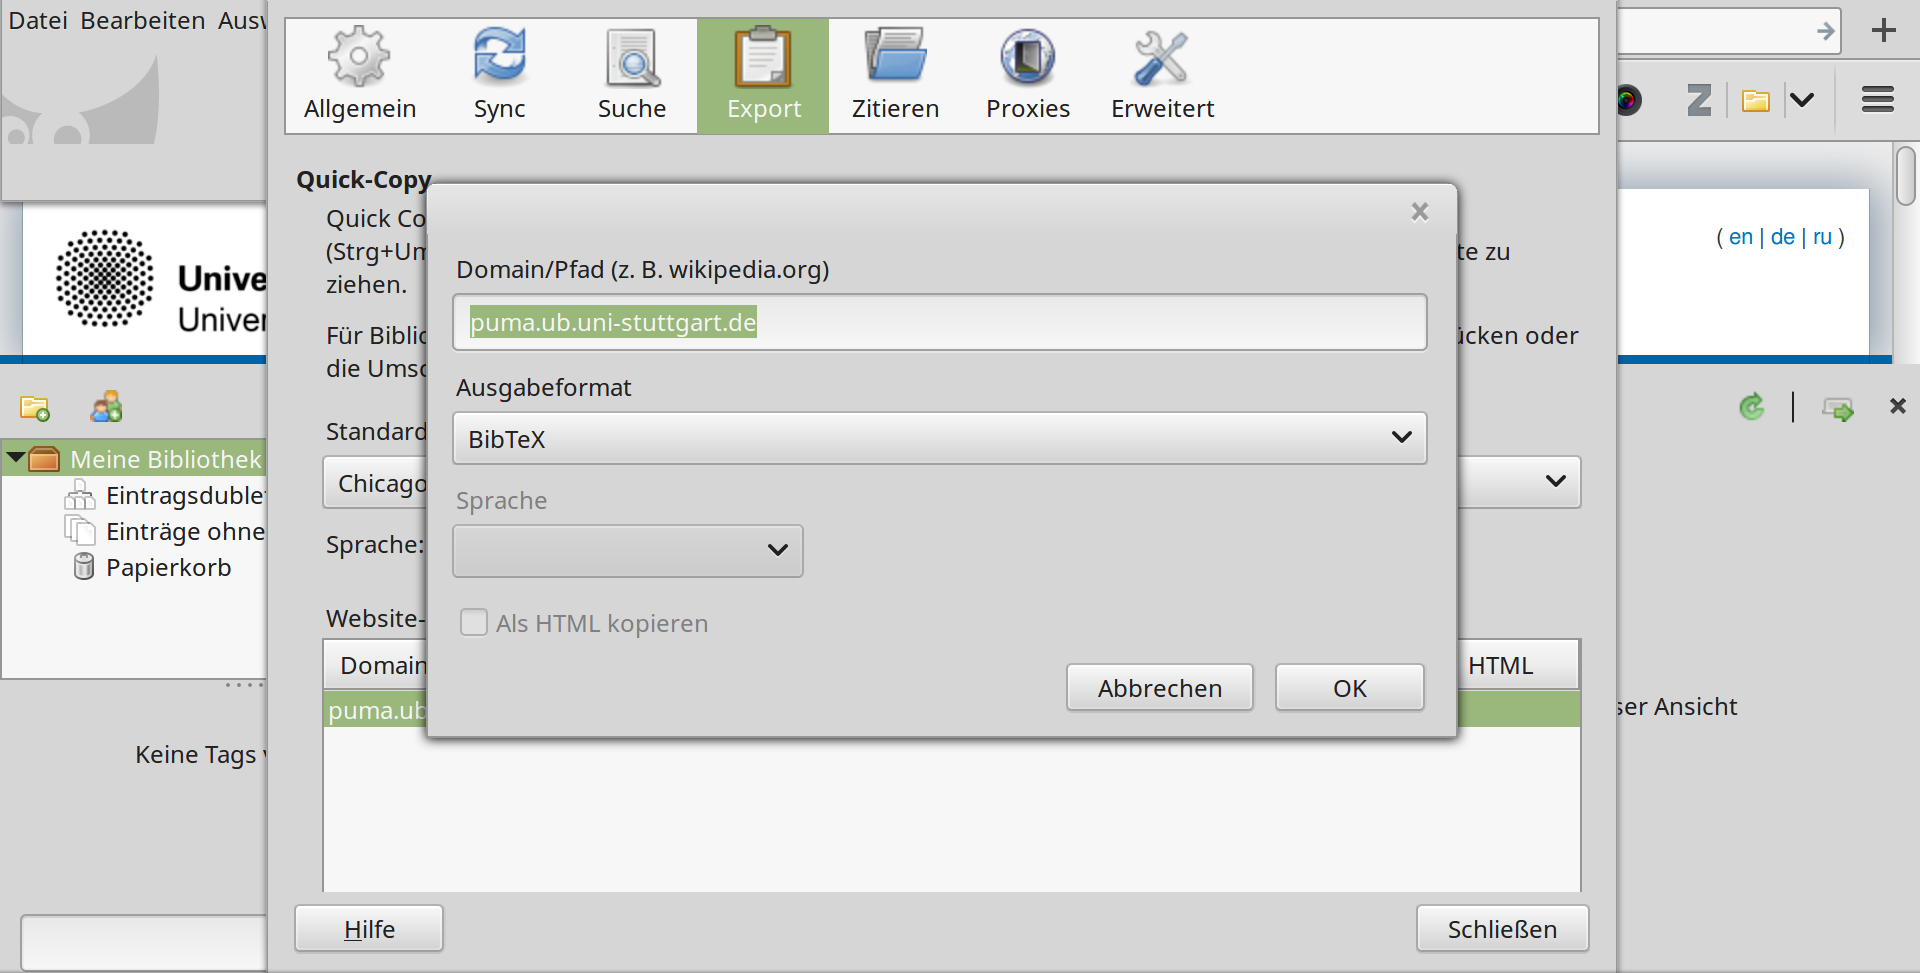
\includegraphics[width=9cm]{Bilder/Kapitel7/Zotero_Menuepunkt_Export}}
 \caption{Menüpunkt Export}
 \label{fig:menueExport}
\end{figure} 
    
Nachdem die Konfiguration vorgenommen wurde, können die Publikationen nach PUMA importiert werden. 
Dazu im Reiter \enquote{BibTex\index{BibTex}/EndNote\index{EndNote}-Schnipsel}. In das Feld \enquote{Auswahl} den entsprechenden Eintrag aus der Zotero-Bibliothek durch Drag und Drop hineinziehen.
\begin{figure}[h!]
 \centering
 \fbox{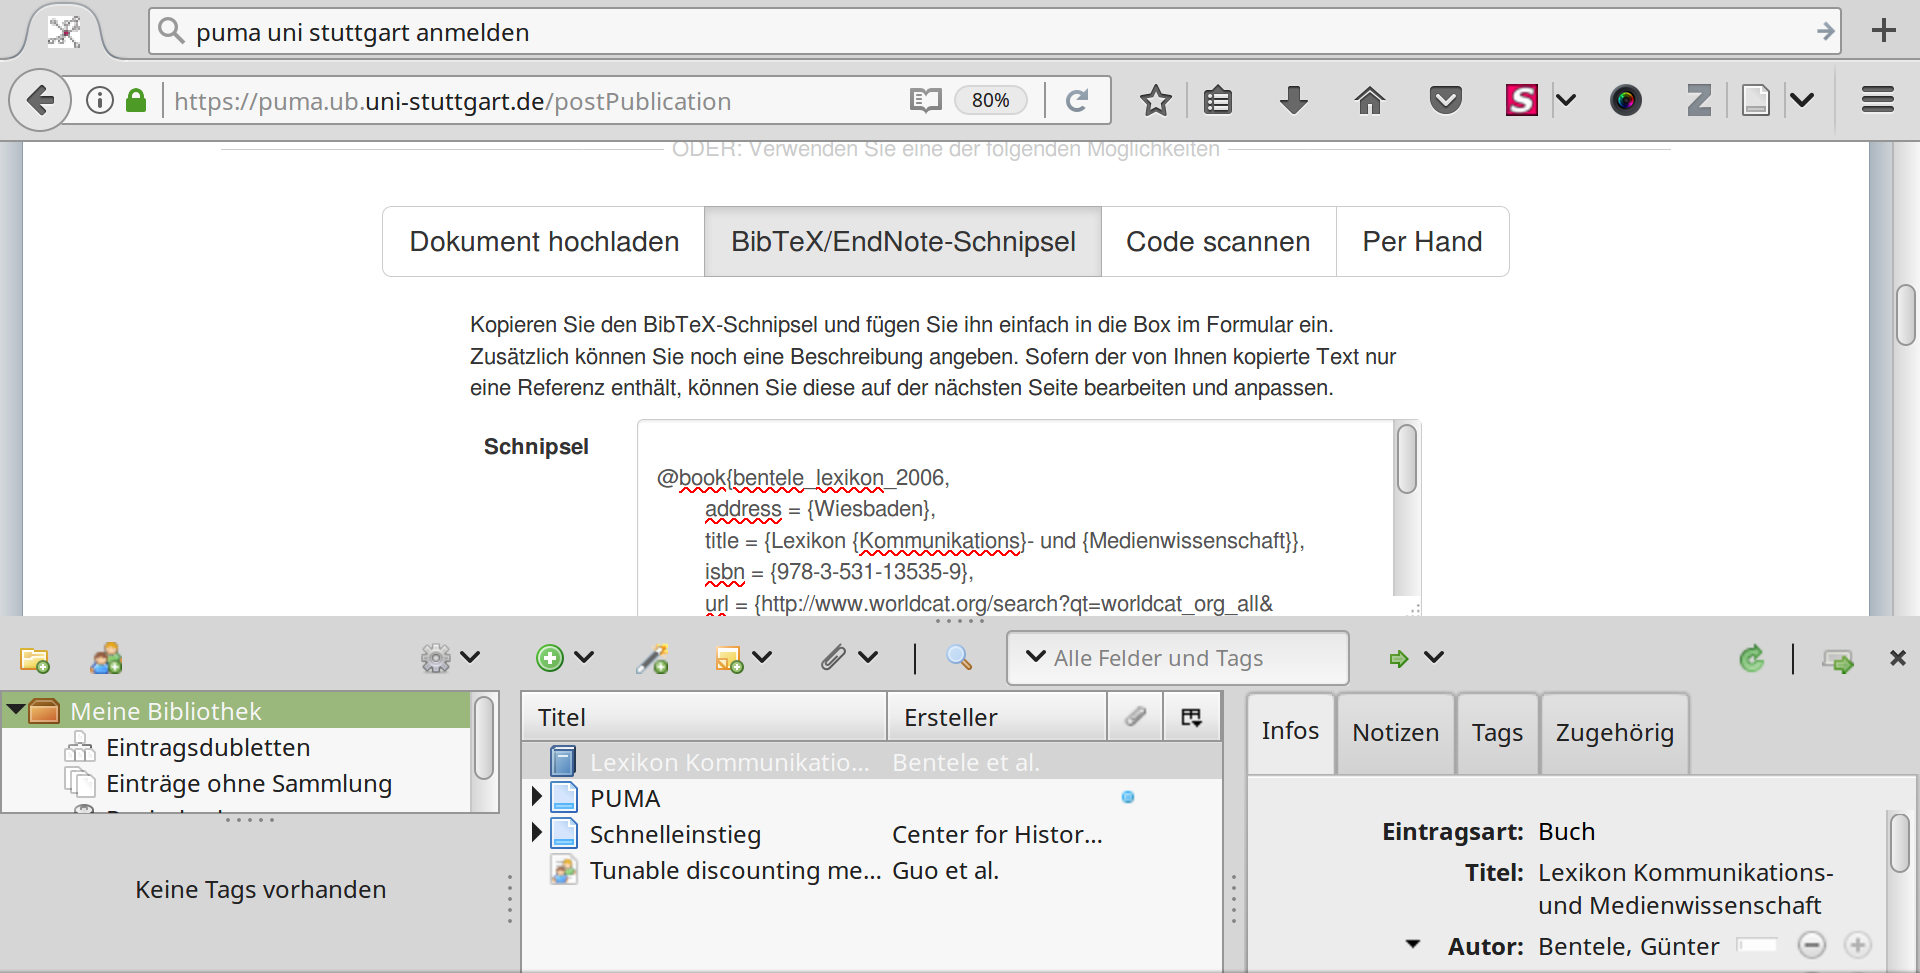
\includegraphics[width=10cm]{Bilder/Kapitel7/Zu_PUMA_importieren}}
 \caption{Zu PUMA importieren}
 \label{fig:zuPumaImportieren}
\end{figure}

\subsubsection*{Bib-TeX-Export aus Citavi\index{Import!Citavi}}\label{sss:importCitavi} 
Bei Citavi\index{Citavi} oben rechts über \enquote{Datei} im Dropdown-Menü \enquote{Exportieren} auswählen. Die gewünschten Einträge markieren und als Export-Format \enquote{BibTex} angeben.
    
\begin{figure}[h!]
 \centering
 \fbox{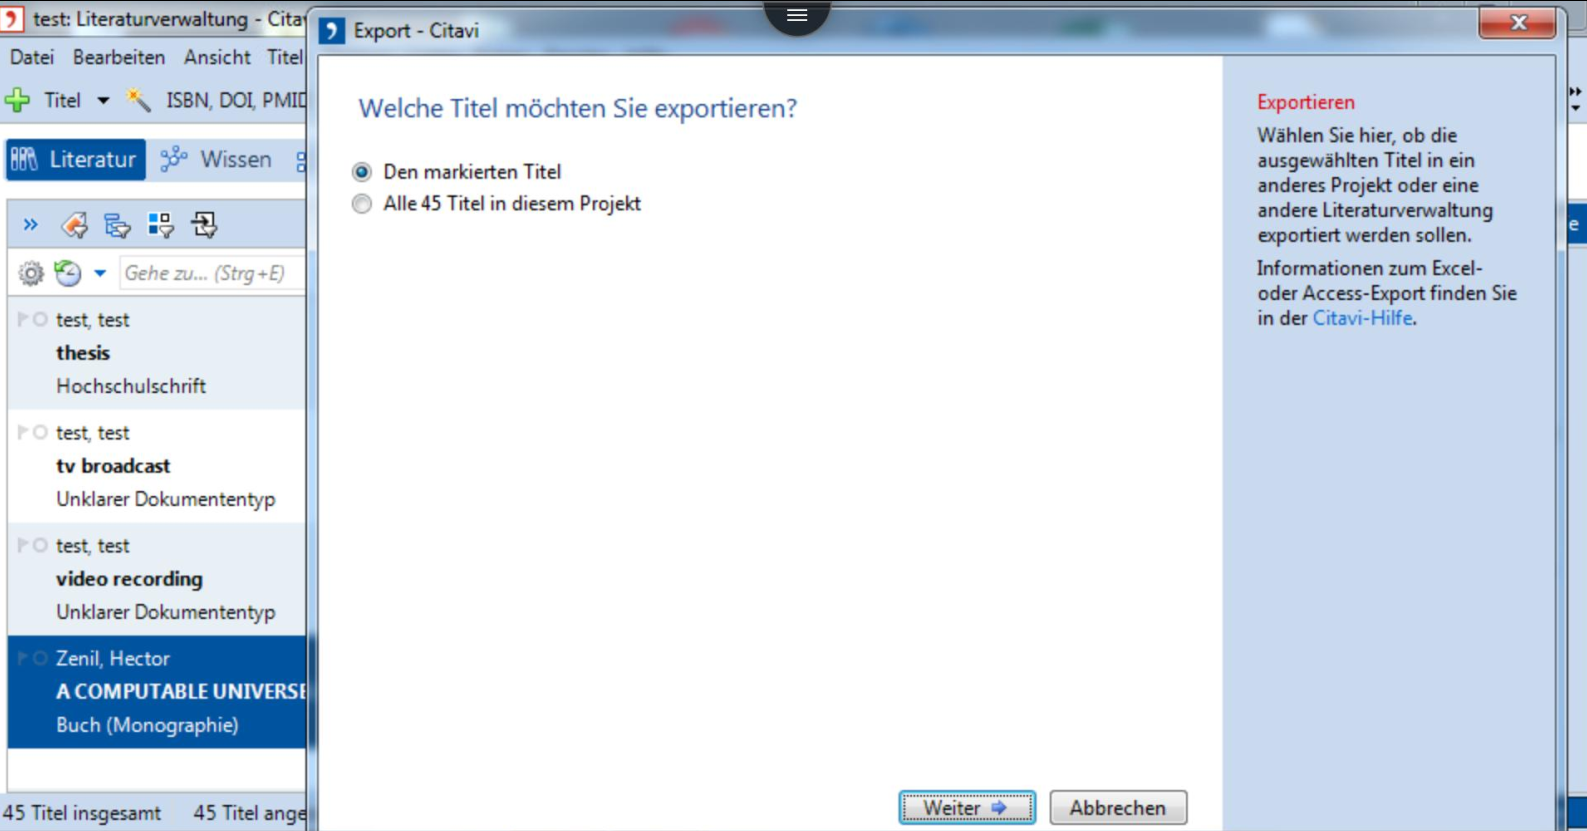
\includegraphics[width=9cm]{Bilder/Kapitel7/Citavi_Schritt2}}
 \caption{Auswählen der zu exportierenden Artikel}
 \label{fig:exportierendenArtikelAuswaehlen}
\end{figure}

  
\begin{figure}[h!]
 \centering
 \fbox{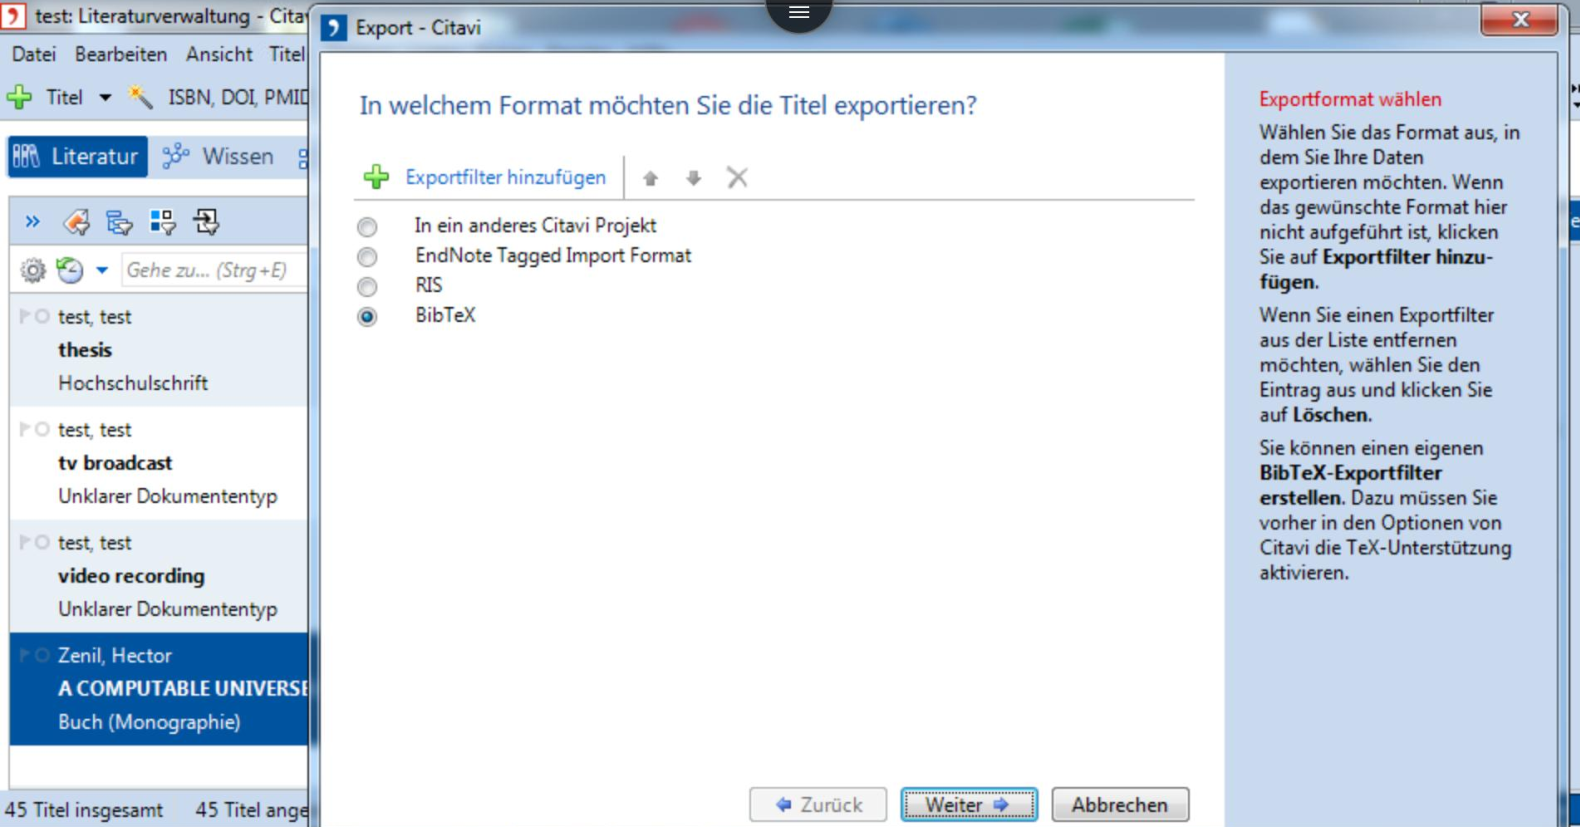
\includegraphics[width=9cm]{Bilder/Kapitel7/Citavi_Schritt3}}
 \caption{Export-Format festlegen}
 \label{fig:exportFormatFestlegen}
\end{figure}

 Als Speicherort \enquote{Textdaten in der Zwischenablage speichern} wählen und die Export-Vorlage unter dem Namen \textit{BibTex} speichern.
   
\begin{figure}[h!]
 \centering
 \fbox{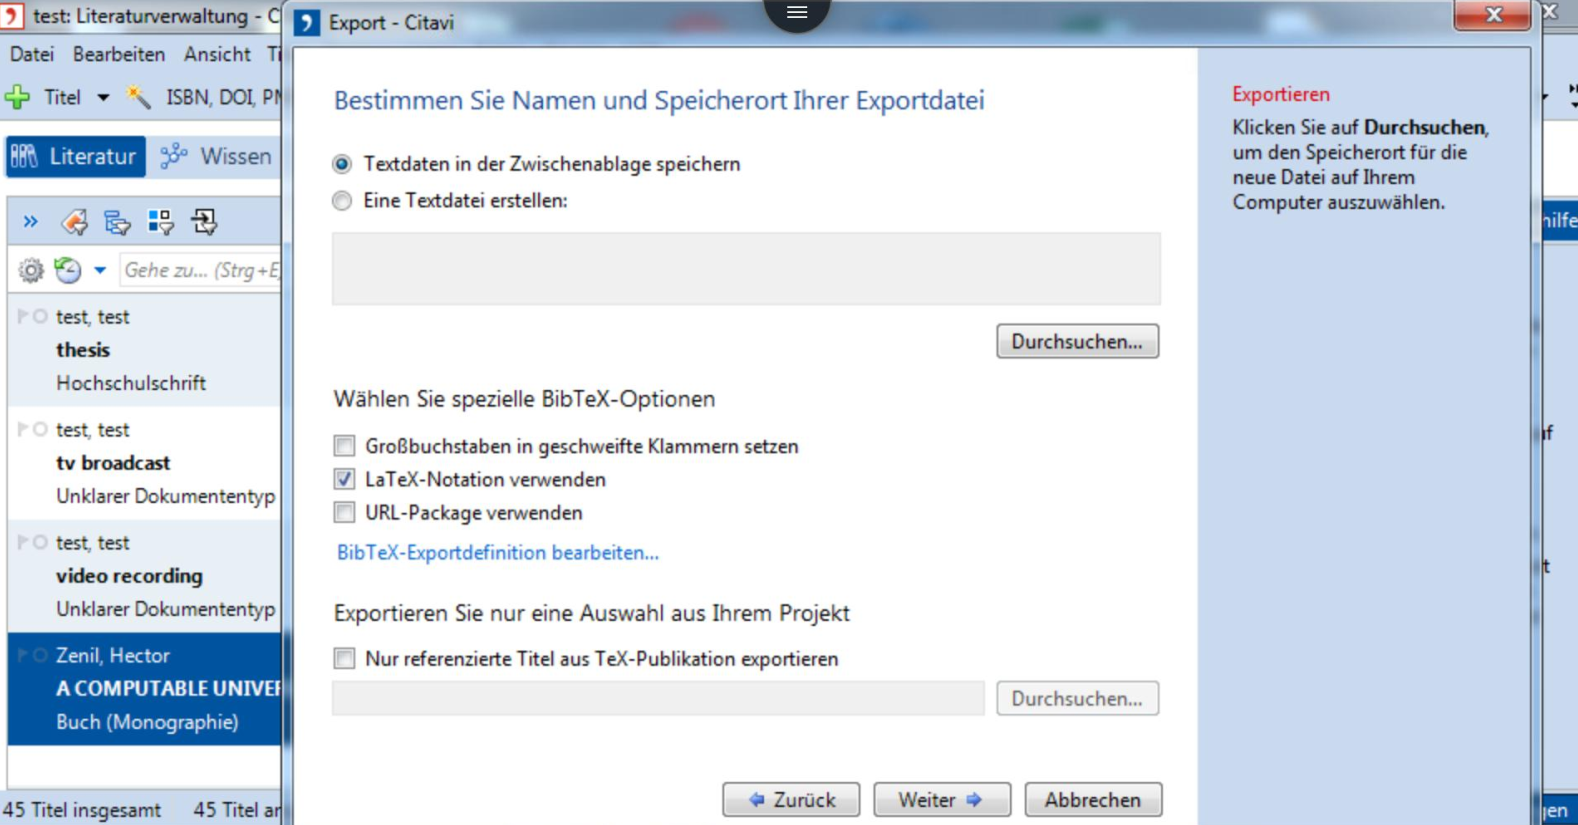
\includegraphics[width=9cm]{Bilder/Kapitel7/Citavi_Schritt4}}
 \caption{Speicherort}
 \label{fig:speicherort}
\end{figure}

\begin{figure}[h!]
 \centering
 \fbox{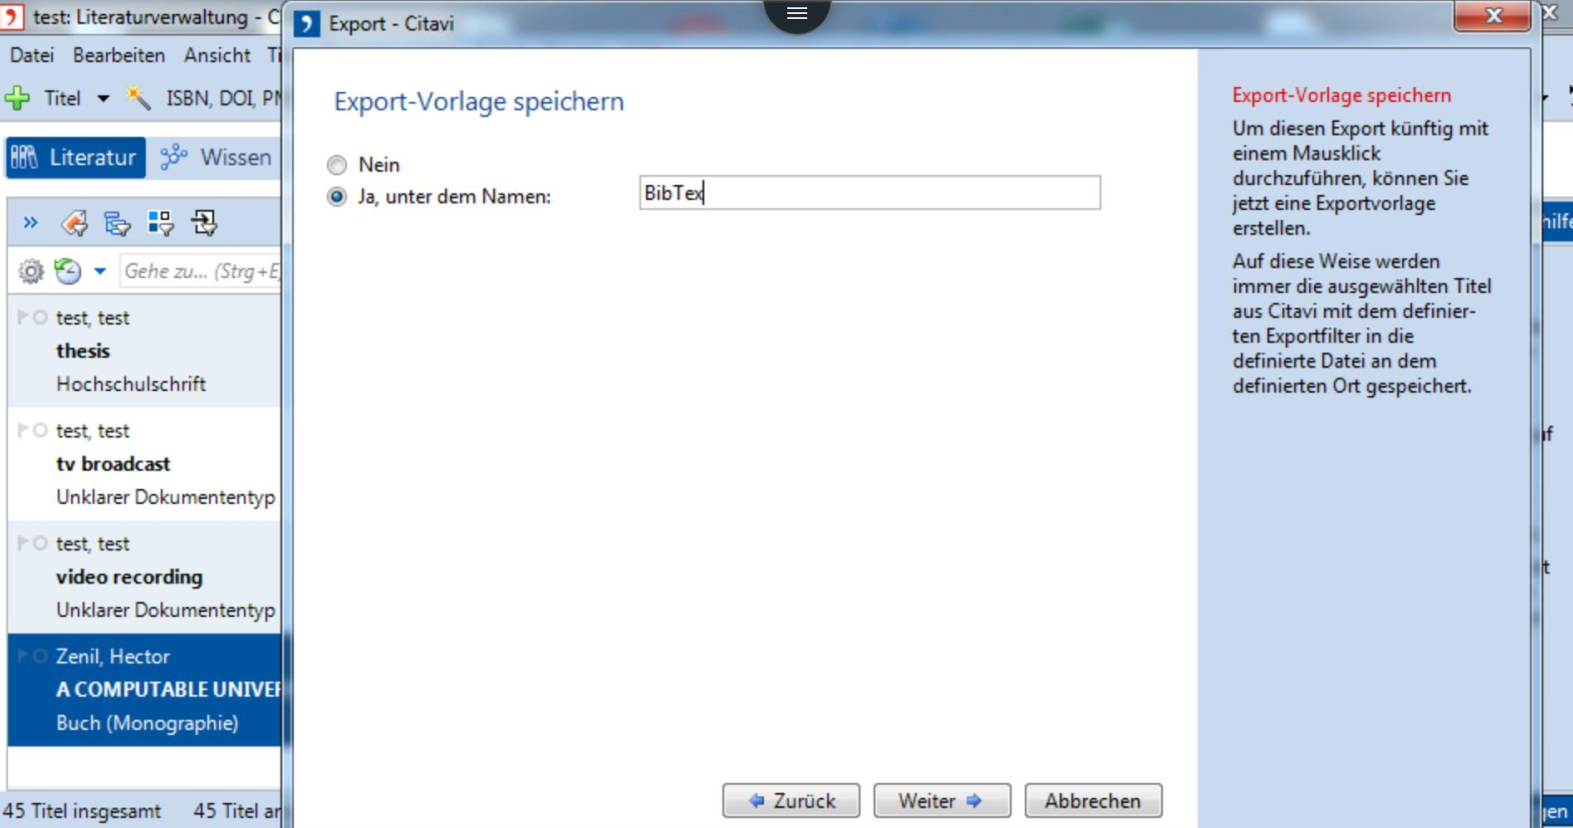
\includegraphics[width=9cm]{Bilder/Kapitel7/Citavi_Schritt5}}
 \caption{Export-Vorlage speichern}
 \label{fig:exportVorlageSpeichern}
\end{figure}

Die exportierte Daten befinden sich nun in der Zwischenablage. Wie in \nameref{subsec:bibtexImportieren} beschrieben fortfahren, um die Daten endgültig nach PUMA zu importieren.\newline

\subsubsection{Import aus JabRef\index{Import!JabRef}\index{JabRef}}\label{sss:importJabRef}
Mit der rechten Maustaste auf die Publikation, die nach PUMA importiert werden soll klicken.
Diese in die Zwischenablage im Export-Format BibTex kopieren.


\section{RSS-Feed abonnieren} 
\label{sec:rssFeedAbonnieren}
RSS\index{RSS} (engl. Really Simple Syndication)-Feeds informieren über Veränderungen auf Websites. In PUMA können eigene oder fremde Publikations-/~Lesezeichenlisten als RSS-Feed abonniert werden. Dies funktioniert auch mit Publikationslisten von Gruppen. Dazu über das Exportzeichen in der Publikations-/~Lesezeichenspalte, die abonniert werden soll auf \enquote{RSS} klicken. 

\begin{figure}[h!]
 \centering
 \fbox{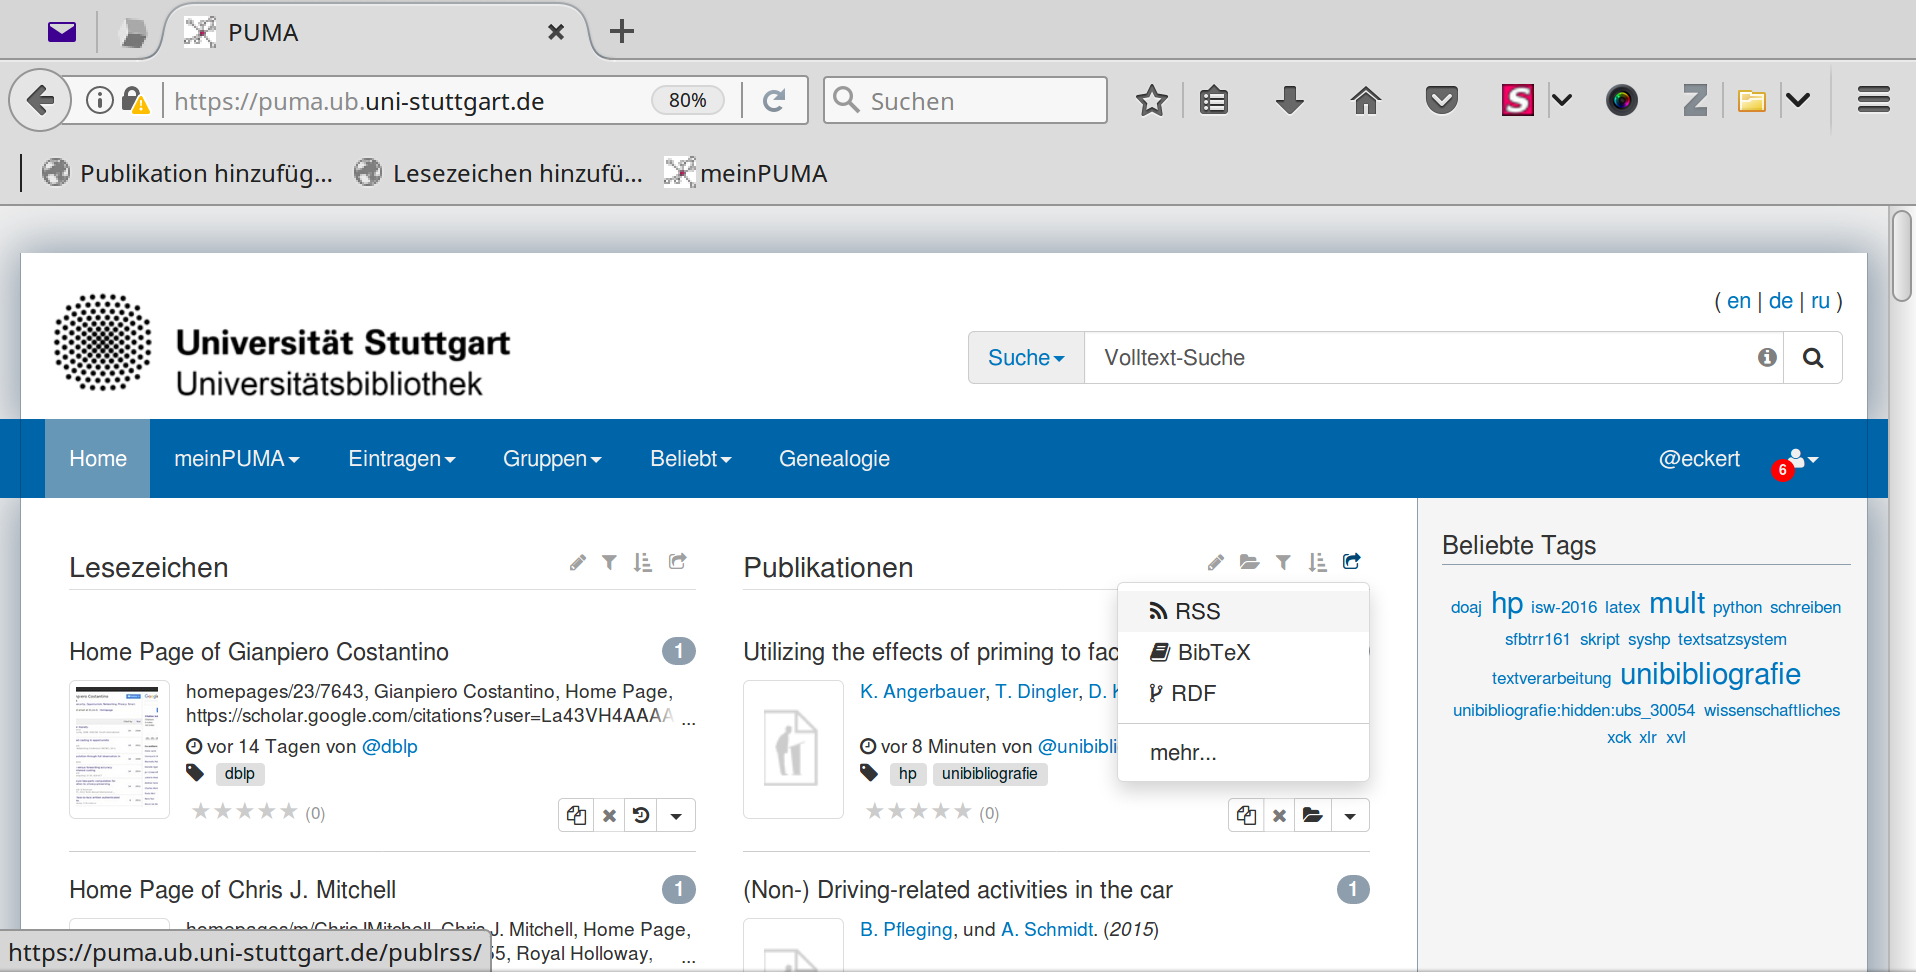
\includegraphics[width=10cm]{Bilder/Kapitel7/RSS-feed_abonnieren}}
 \caption{RSS-Feed abonnieren}
 \label{fig:rssFeedAbbonnieren}
\end{figure}

\begin{figure}[h!]
 \centering
 \fbox{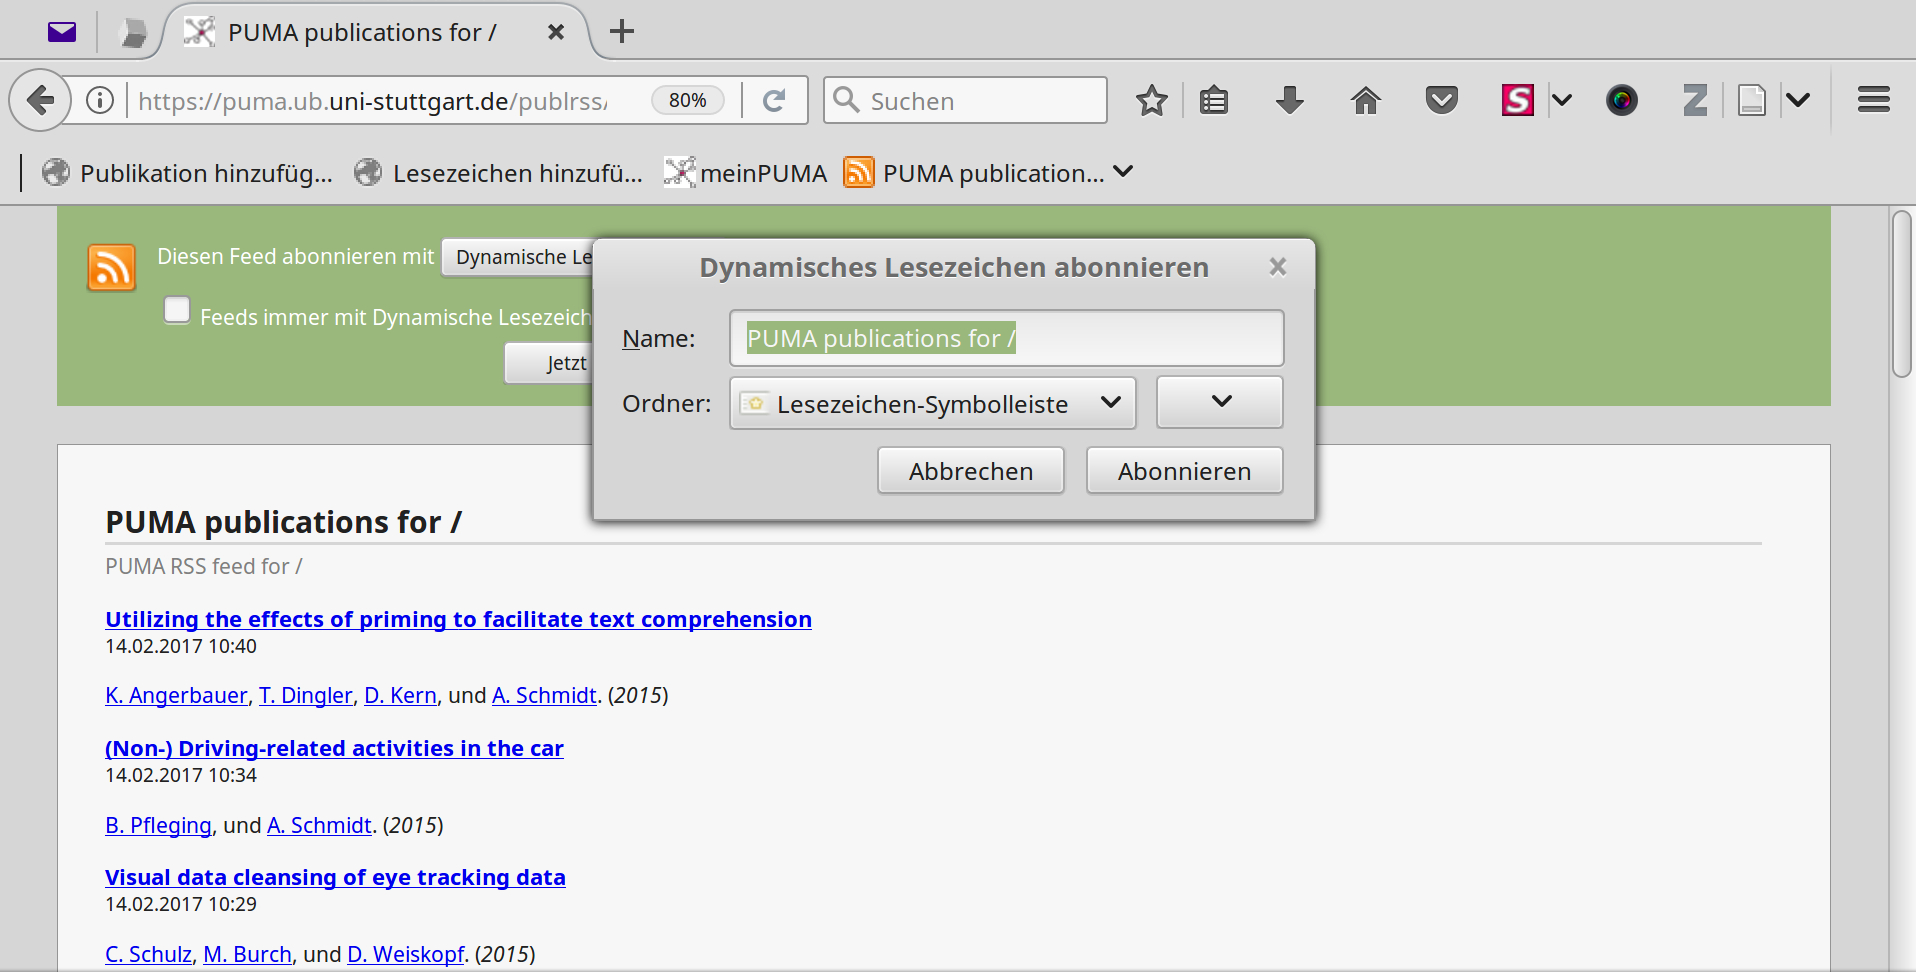
\includegraphics[width=11cm]{Bilder/Kapitel7/RSS_dynamisches_Lesezeichen}}
 \caption{Das dynamische Lesezeichen}
 \label{fig:dynamischesLesezeichen}
\end{figure}

\begin{figure}[h!]
 \centering
 \fbox{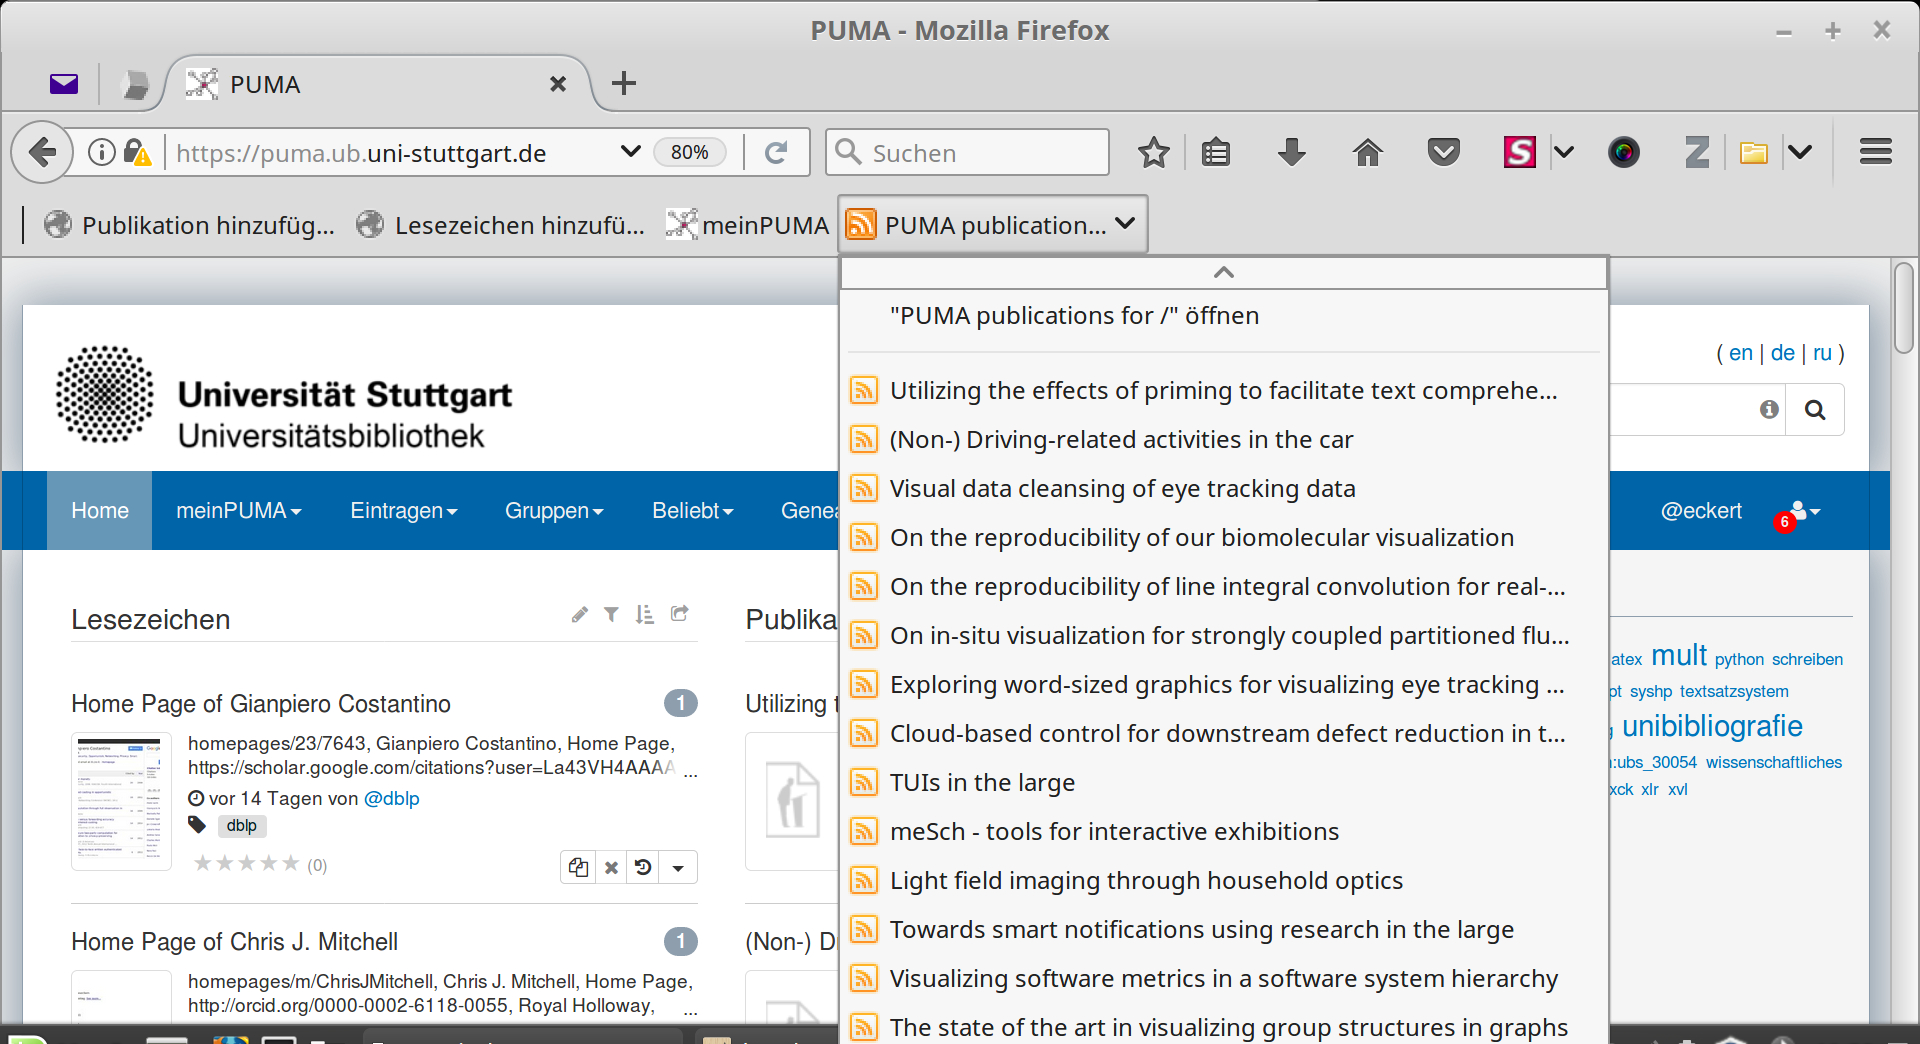
\includegraphics[width=11cm]{Bilder/Kapitel7/RSS-Reader}}
 \caption{Der RSS-Reader}
 \label{fig:rssReader}
\end{figure}

\section{Universitätsbibliografie\index{Unibibliografie}}
\label{sec:unibibliografie}
Die Universitätsbibliografie (kurz: Unibibliografie) bietet eine möglichst vollständige Übersicht über die Publikationen, die an der Universität Stuttgart veröffentlicht werden. Seit 2015 werden sämtliche Publikationen aller wissenschaftlichen Mitglieder (nach §9 LHG) der Universität Stuttgart angezeigt, die während und ggf. nach ihrer Zugehörigkeit zur Universität verfasst bzw. herausgegeben, öffentlich und dauerhaft verfügbar gemacht wurden.\newline\newline
Geführt wird die Unibibliografie der Universität Stuttgart über PUMA. Für die Mitglieder der Universität besteht die Möglichkeit, Publikationen über PUMA zu melden. Die Universitätsbibliothek bearbeitet die Datensätze und veröffentlicht diese Publikationsmetadaten in der Gruppe \textit{unibibliografie} in PUMA. Die Einträge dieser Gruppe können über \texttt{/group/unibibliografie} eingesehen und über \texttt{/export/group/unibibliographie} in viele verschiedene Formate exportiert werden (siehe auch \autoref{sss:nachGruppe} und \autoref{subsec:export}). Weitere Informationen gibt es auf der Homepage der Universitätsbibliothek Stuttgart. \footnote{\url{http://www.ub.uni-stuttgart.de/forschen-publizieren/unibibliografie/}}
\section{OPUS}
\label{sec:opus}
OPUS ist der Dokumentenserver (das institutionelle Repositorium) der Universität Stuttgart. Alle Angehörigen der Universität Stuttgart können über OPUS ihre Dokumente, die von dauerhaftem Interesse für Forschung und Lehre sind, online im Sinne von Open Access\index{Open Access} veröffentlichen. Durch diesen Schritt werden Publikationen im Internet langfristig und weltweit frei zugänglich. Zudem werden die Veröffentlichungen auch in Bibliothekskatalogen, Datenbanken und allen gängigen Suchmaschinen nachgewiesen und somit die Sichtbarkeit der Publikationen deutlich erhöht. Die Zitierfähigkeit der Veröffentlichungen wird durch eine dauerhafte, stabile Internet-Adresse (Persistent Identifier) garantiert.
\newline\newline
Geplant ist die Möglichkeit, aus PUMA direkt in OPUS\index{OPUS} zu veröffentlichen. Bei der Verwendung des \tags \textit{myown} (\autoref{sss:systemtags}) wird die Veröffentlichung auf OPUS angeboten.  

%\subsection{OPUS und PUMA}
%\label{subsec:opusPuma}
%Beim Eintragen einer Veröffentlichung/Publikation in PUMA wird die eigene Veröffentlichung mit \textit{myown} getaggt. Sie werden von PUMA gefragt, ob Sie auf OPUS veröffentlichen wollen. Wenn Sie diese Frage mit \enquote{Ja} bestätigen, wird eine SWORD-Datenverbindung\index{SWORD} zur Sherpa/Romeo-Liste\index{Sherpa/Romeo-Liste} hergestellt. Diese zeigt an, was die Verlage im Bezug auf die Veröffentlichung erlauben. Ist das Hochladen \enquote{grün}, so wird die Veröffentlichung auf OPUS  hochgeladen (so genanntes \enquote{Self Archiving}).
%\newline \newline
%Die Sherpa/Romeo-Liste\footnote{\url{http://www.sherpa.ac.uk/romeo/index.php}} ist eine Datenbank in Manchester, über die die Verlagskonditionen für Zweitveröffentlichungen abgefragt werden können. Bei deutschen Verlagen gilt ein Zeitfenster von 12 Monate nach Erstveröffentlichung, bevor die Autoren eine Zweitveröffentlichung machen können (Grüner Weg des Open Access). Bei Verlagen im Ausland gelten z. T. deutlich höhere Schutzfristen.
\section{DBLP}
\label{dblp}
Das Digital Bibliography \& Library Project (DBLP\index{DBLP}; zu deutsch: Digitales Bibliographie- und Bibliotheksprojekt) betreibt eine online verfügbare bibliographische Datenbank. In der Sammlung befinden sich mehr als 3 Mio. unterschiedliche wissenschaftliche Publikationen aus dem Bereich Informatik.\newline
PUMA und BibSonomy sind mit der DBLP-Datenbank verbunden. Die Datenbank wird mehrmals wöchentlich aktualisiert und stellt PUMA und BibSonomy Publikationen zur Nachnutzung zur Verfügung. \newline
Die Nutzer können so Einträge der DBLP-Datenbank mit ein paar Klicks in die eigene Sammlung übernehmen. 
